\documentclass{article}
\usepackage{tikz}
\usepgflibrary{shapes.symbols}
\usetikzlibrary{arrows.meta, shapes.geometric}
\begin{document}
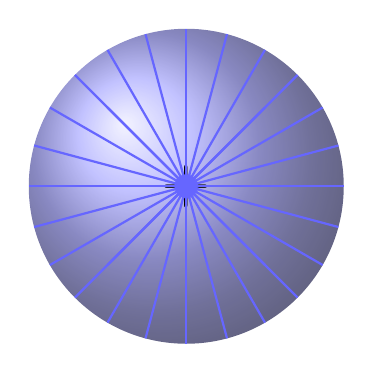
\begin{tikzpicture}[xshift=-1cm]
% Shaded sphere (3D-like)
\shade[ball color=blue!40, opacity=0.8] (0,0) circle (2cm);

% Central monopole (+ symbol)
\node[inner sep=0pt] at (0,0) {\scalebox{2}{\textbf{+}}};

% Spherical field lines (multiple radial angles)
\foreach \angle in {0, 15,...,345} {
    \draw[stealth-, thick, color=blue!60] (0,0) -- (\angle:2cm);
}

% Optional: Add perspective effect with extra lines
\draw[thick, color=blue!60] (0,0) -- (2,0); % Right
\draw[thick, color=blue!60] (0,0) -- (-2,0); % Left
\draw[thick, color=blue!60] (0,0) -- (0,2); % Up
\draw[thick, color=blue!60] (0,0) -- (0,-2); % Down
\draw[thick, color=blue!60] (0,0) -- (1,1); % Diagonal right-up
\draw[thick, color=blue!60] (0,0) -- (1,-1); % Diagonal right-down
\draw[thick, color=blue!60] (0,0) -- (-1,1); % Diagonal left-up
\draw[thick, color=blue!60] (0,0) -- (-1,-1); % Diagonal left-down
\end{tikzpicture}
\end{document}
